\begin{figure}[htbp]
  \centering
  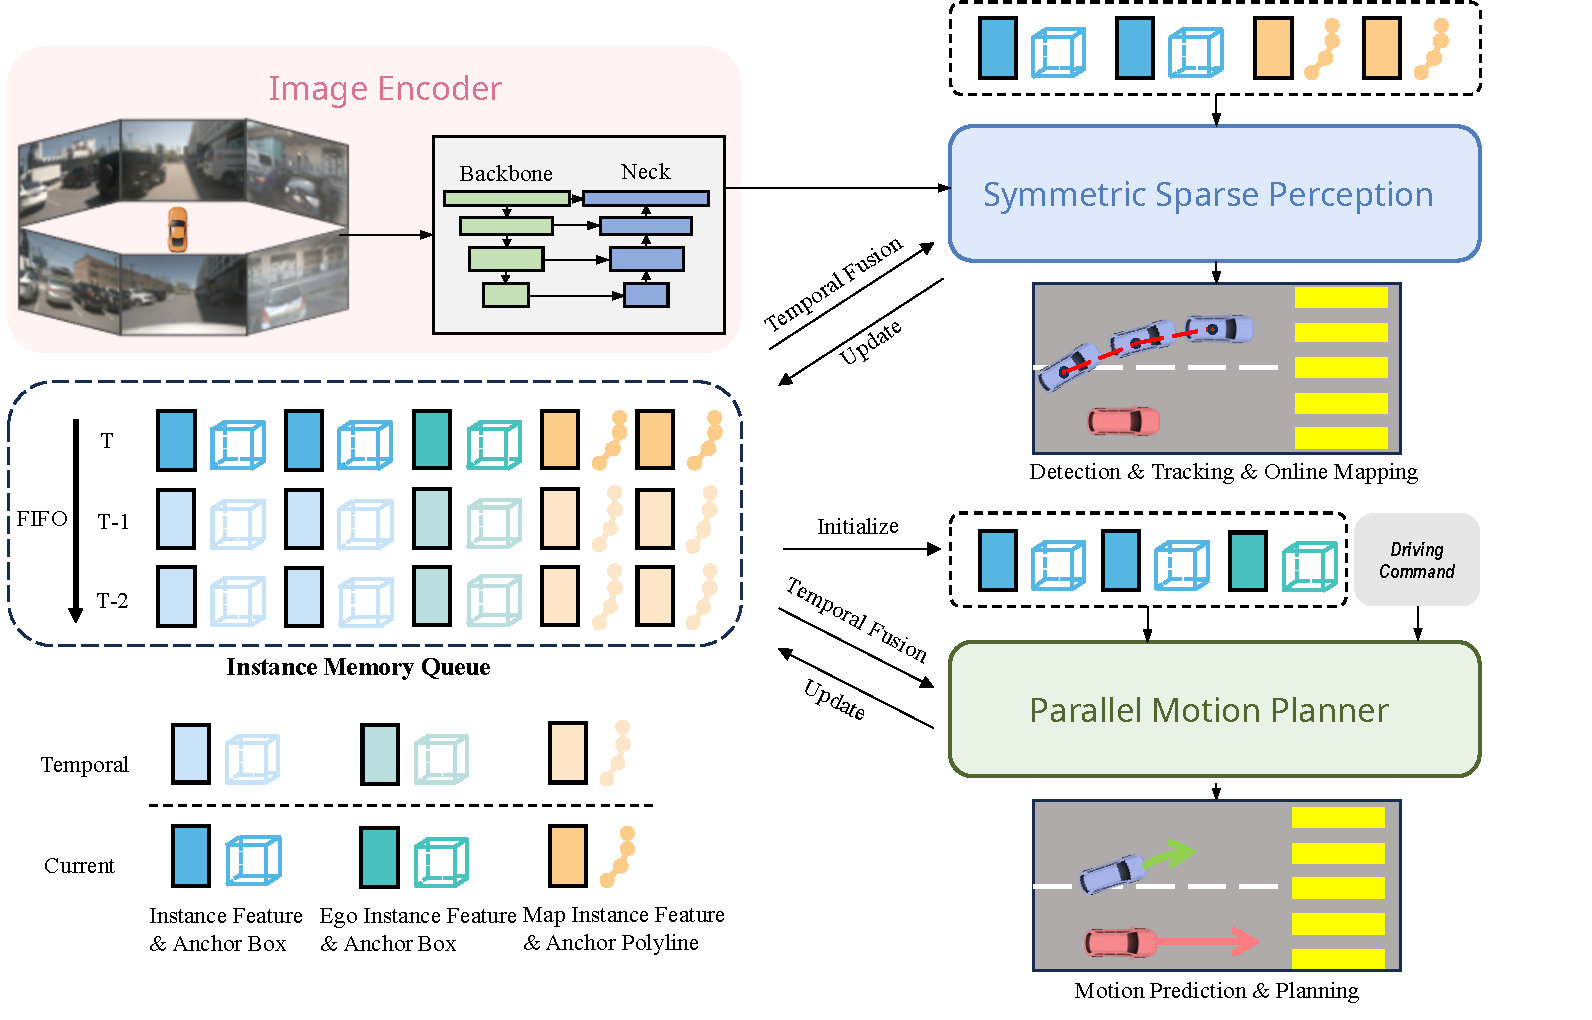
\includegraphics[width=0.8\linewidth]{Figures/overview_.pdf}
  \caption{Overview of SparseDrive. SparseDrive first encodes multi-view images into feature maps, then learns sparse scene representation through symmetric sparse perception, and finally perform motion prediction and planning in a parallel manner. An instance memory queue is devised for temporal modeling.}
  \label{fig:overview}
\end{figure}

\section{Method}
\subsection{Overview}
The overall framework of SparseDrive is depicted in Fig. \ref{fig:overview}. Specifically, SparseDrive is consisted of three parts: image encoder, symmetric sparse perception and parallel motion planner. Given multi-view images, the image encoder, including a backbone network and a neck, first encodes images to multi-view multi-scale feature maps $I=\left\{I_s \in \mathbb{R}^{N \times C \times H_s \times W_s} | 1 \leq s \leq S \right\}$, where $S$ is the number of scales and $N$ is the number of camera views. In symmetric sparse perception module, the feature maps $I$ are aggregated into two groups of instances to learn the sparse representation of the driving scene. These two groups of instances, representing surrounding agents and map elements respectively, are fed into parallel motion planner to interact with an initialized ego instance. The motion planner predicts multi-modal trajectories of surrounding agents and ego vehicle simultaneously, and selects a safe trajectory as the final planning result through hierarchical planning selection strategy.

\subsection{Symmetric Sparse Perception}
As shown in Fig. \ref{fig:sparse_perception}, the model structure of sparse perception module exhibits a structural symmetry, unifying detection, tracking and online mapping together.

\paragraph{Sparse Detection.}
Surrounding agents are represented by a group of instance features $F_d \in \mathbb{R}^{N_d \times C}$ and anchor boxes $B_d \in \mathbb{R}^{N_d \times 11}$, where $N_d$ is the number of anchors and $C$ is the feature channel dimension. Each anchor box is formatted  with location, dimension, yaw angle and velocity:
% \[ \left\{x,y,z,\mathrm{ln }w, \mathrm{ln}h, \mathrm{ln}l, \mathrm{sin}yaw, \mathrm{cos}yaw, vx, vy, vz\right\}. \]
\[ \left\{ x, y, z, \ln w, \ln h, \ln l, \sin{yaw}, \cos{yaw}, vx, vy, vz\right\}. \]

The sparse detection branch consists of $N_{dec}$ decoders, including a single non-temporal decoder and $N_{dec}-1$ temporal decoders. Each decoder takes feature maps $I$, instance features $F_d$ and anchor boxes $B_d$ as input, outputs updated instance features and refined anchor boxes. The non-temporal decoder takes randomly initialized instance as input, while the input for temporal decoder come from both current frame and historical frame. Specifically, the non-temporal decoder includes three sub-modules: deformable aggregation, feedforward network (FFN) and the output layer for refinement and classification. The deformable aggregation module generates fixed or learnable keypoints around the anchor boxes $B_d$ and projects them to feature maps $I$ for feature sampling. The instance features $F_d$ are updated by summation with sampled features, and are responsible for predicting the classification scores and the offsets of anchor boxes in the output layer. The temporal decoders have two additional multi-head attention layers: the temporal cross-attention between temporal instances from last frame and current instances, and the self-attention among current instances. In multi-head attention layer, the anchor boxes are transformed into high-dimensional anchor embedding $E_d \in \mathbb{R}^{N_d \times C}$, and serve as the positional encoding.

\begin{figure}[htbp]
  \centering
  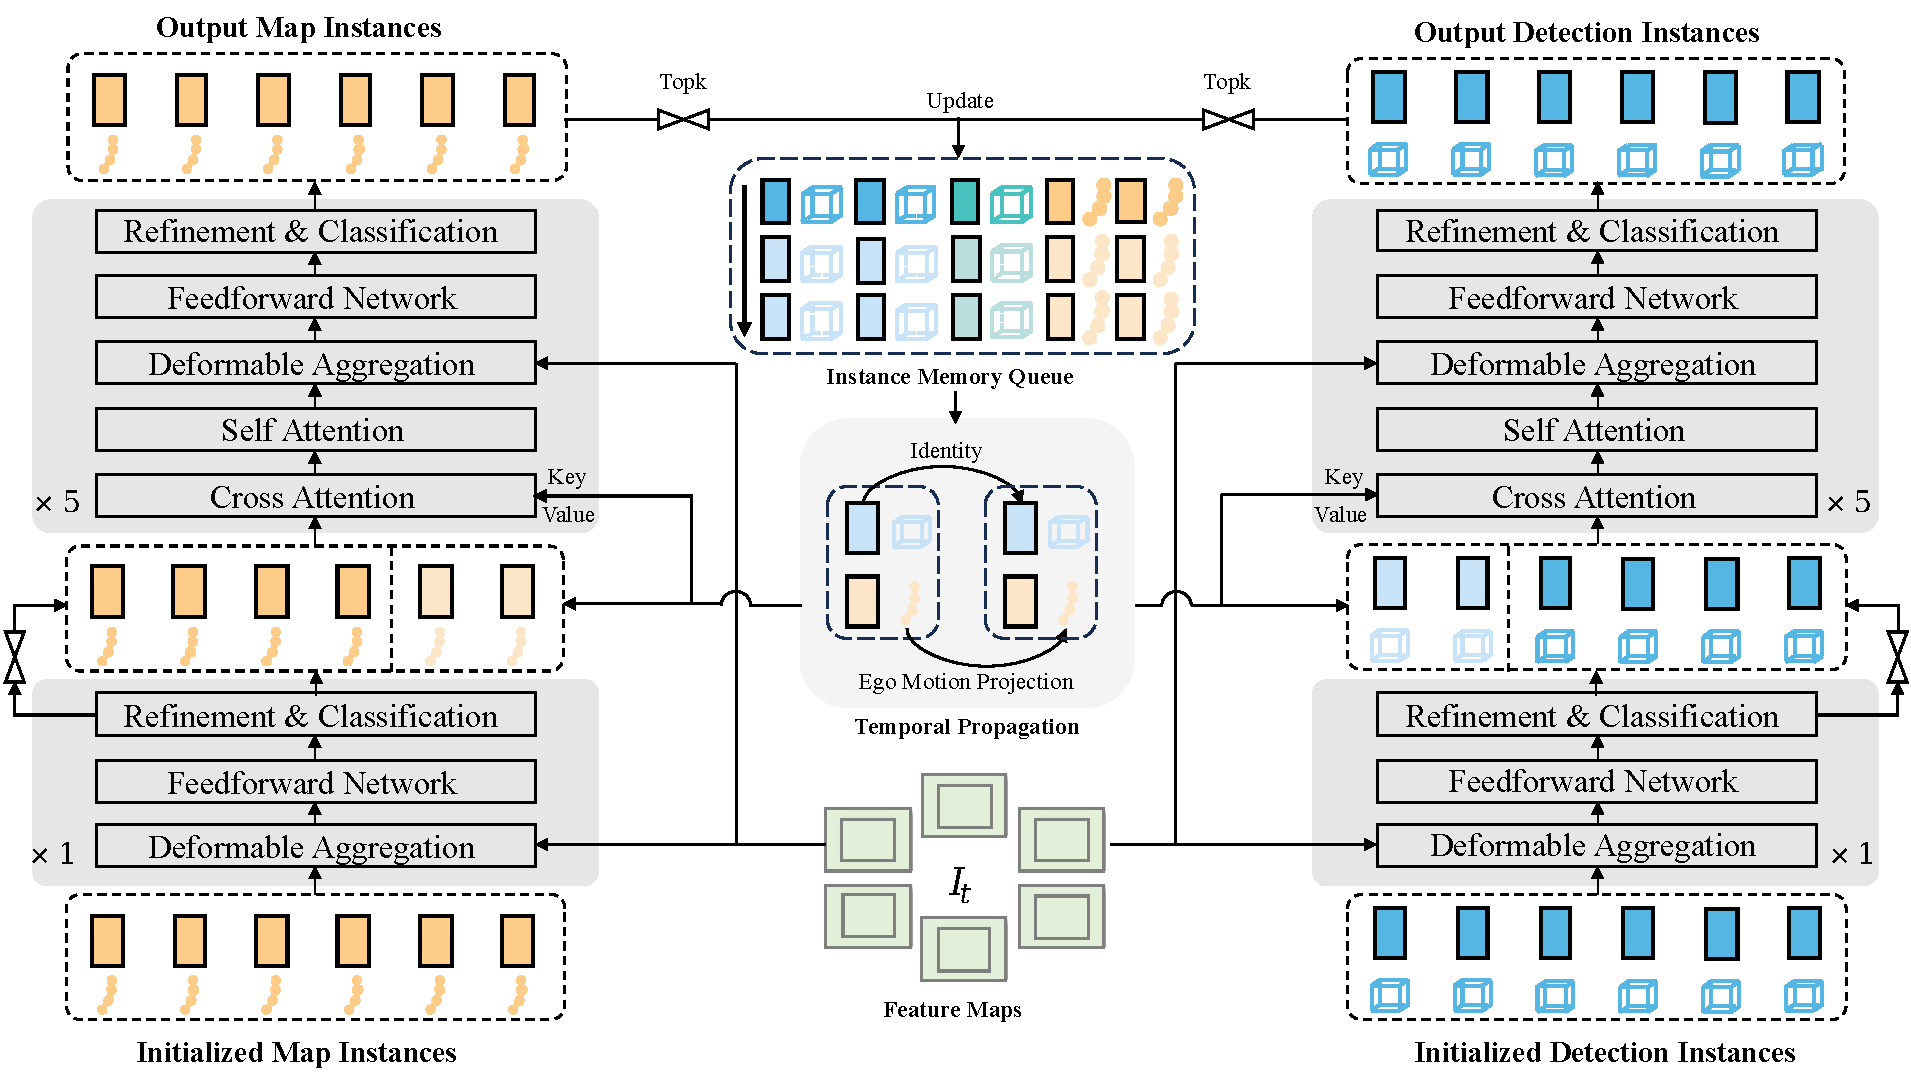
\includegraphics[width=0.85\linewidth]{Figures/sparse_perception_.pdf}
  \caption{Model architecture of symmetric sparse perception, which unifies detection, tracking and online mapping in a symmetric structure.}
  \label{fig:sparse_perception}
\end{figure}

\paragraph{Sparse Online Mapping.}
Online mapping branch shares the same model structure with detection branch except different instance definition. For static map element, the anchor is formulated as a polyline with $N_p$ points: \[ \left\{x_{0},y_{0},x_{1},y_{1},...,x_{N_p-1},y_{N_p-1} \right\}. \] 

Then all the map elements can be represented by map instance features $F_m \in \mathbb{R}^{N_m \times C}$ and anchor polylines $L_m \in \mathbb{R}^{N_m \times N_p \times 2}$, where $N_m$ is the number of anchor polylines.

\paragraph{Sparse Tracking.}
For tracking, we follow the ID assignment process of Sparse4Dv3\cite{sparse4dv3}: once the detection confidence of an instance surpasses a threshold $T_{thresh}$, it is locked onto a target and assigned with an ID, which remains unchanged throughout temporal propagation. This tracking strategy does not need any tracking constraints, resulting in an elegant and simple symmetric design for sparse perception module.

\subsection{Parallel Motion Planner}
As shown in Fig. \ref{fig:motion_planner}, the parallel motion planner consists of three parts: ego instance initialization, spatial-temporal interactions and hierarchical planning selection.

\paragraph{Ego Instance Initialization.}
Similar to surrounding agents, ego vehicle is represented by ego instance feature $F_e \in \mathbb{R}^{1 \times C}$  and ego anchor box $B_e \in \mathbb{R}^{1 \times 11}$. While ego feature is typically randomly initialized in previous methods, we argue that the ego feature also requires rich semantic and geometric information for planning, similar to motion prediction. However, the instance features of surrounding agents are aggregated from image feature maps $I$, which is not feasible for ego vehicle, since ego vehicle is in blind area of cameras. Thus we use the smallest feature map of front camera to initialize the ego instance feature: 
\begin{equation}
F_e = {\rm AveragePool}(I_{front,S})
\end{equation}
There are two advantages in doing so: the smallest feature map has already encoded the semantic context of the driving scene, and the dense feature map serves as a complementary for sparse scene representation, in case there are some blacklist obstacles, which can not be detected in sparse perception.

For ego anchor $B_e$, the location, dimension and yaw angle can be naturally set, as we are aware of these information of ego vehicle. For velocity, directly initialized from ground truth velocity leads to ego status leakage, as illustrated in \cite{ego}. So we add an auxiliary task to decode current ego status $ES_T$, including velocity, acceleration, angular velocity and steering angle. At each frame, we use the predicted velocity from last frame as the initialization of ego anchor velocity.

\begin{figure}[htbp]
  \centering
  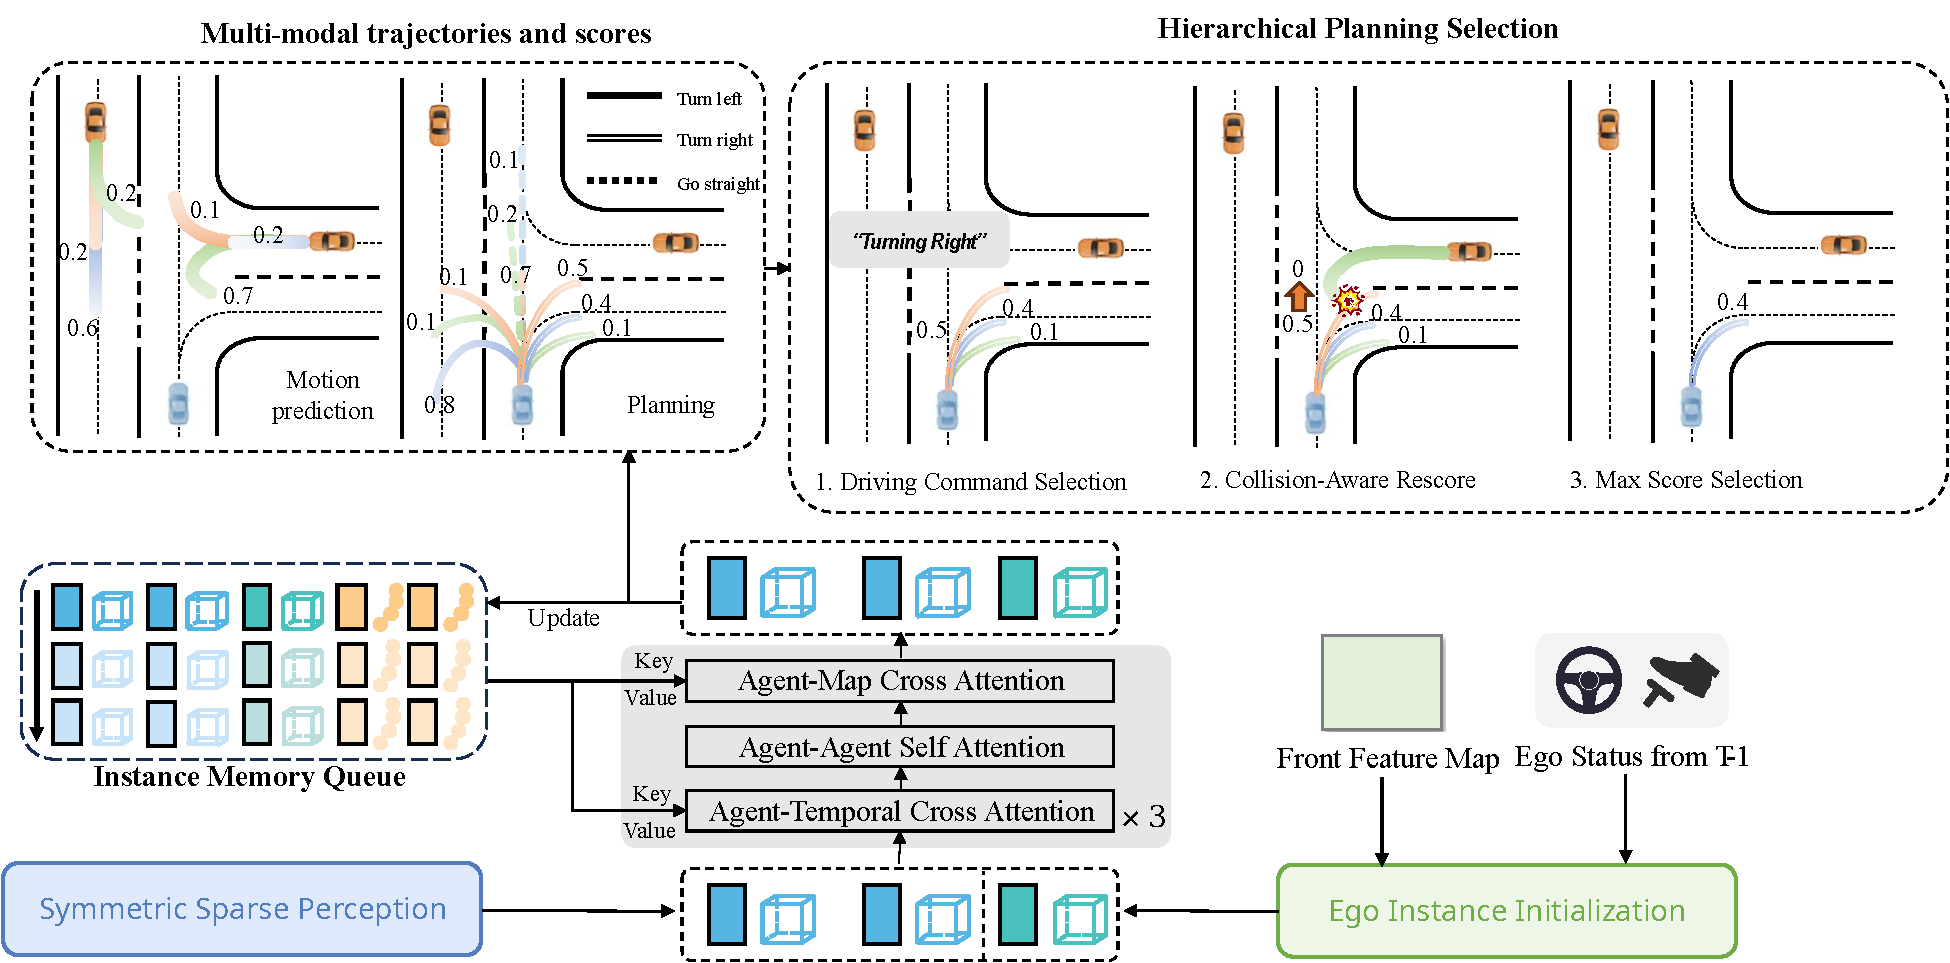
\includegraphics[width=0.83\linewidth]{Figures/motion_planner_.pdf}
  \caption{Model structure of parallel motion planner, which performs motion prediction and planning simultaneously and outputs safe planning trajectory.}
  \label{fig:motion_planner}
\end{figure}

\paragraph{Spatial-Temporal Interactions.}
To consider the high-level interaction between all road agents, we concatenate the ego instance with surrounding agents to get agent-level instances:
\begin{equation}
F_a={\rm Concat}(F_d, F_e), B_a={\rm Concat}(B_d, B_e)
\end{equation}
As the ego instance is initialized without temporal cues, which is important for planning, we devise an instance memory queue with the size of $(N_d+1) \times H$ for temporal modeling, $H$ is the number of stored frames. Then three types of interactions are performed to aggregate spatial-temporal context: agent-temporal cross-attention, agent-agent self-attention and agent-map cross-attention. Note that in temporal cross-attention of sparse perception module, the instances of current frame interact with all temporal instances, which we name as scene-level interaction. While for agent-temporal cross-attention here, we adopt instance-level interaction to make each instance focus on history information of itself.

Then, we predict the multi-modal trajectories $\tau_m \in \mathbb{R}^{N_{d} \times \mathcal{K}_m \times T_{m} \times 2}$, $\tau_p \in \mathbb{R}^{N_{c} \times \mathcal{K}_p \times T_{p} \times 2 }$ and scores $s_m \in \mathbb{R}^{N_{d} \times \mathcal{K}_m}$, $s_p \in \mathbb{R}^{N_{cmd} \times \mathcal{K}_p}$ for both surrounding agents and ego vehicle, $\mathcal{K}_m$ and $\mathcal{K}_p$ are the number of modes for motion prediction and planning, $T_m$ and $T_p$ are the number of future timestamps for motion prediction and planning, and $N_{cmd}$ is the number of driving command for planning. Following the common practice\cite{uniad, vad}, we use three kinds of driving commands: turn left, turn right and go straight. For planning, we additionally predict current ego status from ego instance feature.

\paragraph{Hierarchical Planning Selection.}
Now we have the multi-modal planning trajectory proposals, to select one safe trajectory $\tau_p^* $ to follow, we design a hierarchical planning selection strategy. First, we select a subset of trajectory proposals $\tau_{p,cmd} \in \mathcal{K}_p \times T_{p} \times 2$, corresponding to the high-level command $cmd$. Then, a novel collision-aware rescore module is adopted to ensure safety. With the motion prediction results, we can assess the collision risk of each planning trajectory proposal, for the trajectory with high collision probability, we reduce the score of this trajectory. In practice, we simply set the score of collided trajectory to $0$. Finally, we select the trajectory with the highest score as the final planning output.

\subsection{End-to-End Learning}
\paragraph{Multi-stage Training.}
The training of SparseDrive is divided into two stages. In stage-1, we train symmetric sparse perception module from scratch to learn the sparse scene representation. In stage-2, sparse perception module and parallel motion planner are trained together with no model weights frozen, fully enjoying the benefit of end-to-end optimization. More training details are provided in Appendix \ref{app:training}.

\paragraph{Loss Functions.}
The loss functions include the loss of four tasks, and the loss of each task can be further divider into classification loss and regression loss. For multi-modal motion prediction and planning task, we adopt the winner-takes-all strategy. For planning, there is an additional regression loss for ego status. We also introduce depth estimation as an auxiliary task to enhance the training stability of the perception module. The overall loss function for end-to-end training is: 
\begin{equation}
\mathcal{L}=\mathcal{L}_{det}+\mathcal{L}_{map}+\mathcal{L}_{motion}+\mathcal{L}_{plan}+\mathcal{L}_{depth}.
\end{equation}
More details about loss functions are provided in Appendix \ref{app:loss_func}.
